\documentclass{beamer}
\usepackage[utf8]{inputenc}
\usepackage[T1]{fontenc}

\usepackage{qtree}
\usepackage{dirtree}

\usebackgroundtemplate{
	
\includegraphics[width=\paperwidth,height=\paperheight]{img/background}
}

\title{Chapter 02: Other Classical Techniques}

\begin{document}
	\begin{frame}
		\titlepage
	\end{frame}

	\section{Introduction}
	\begin{frame}{Introduction}
		\begin{itemize}
		    \item Other classical techniques exists
		    \item We will review some of them, and later discuss about comparison
		    \item We will rarely use it, just so you know
		\end{itemize}
	\end{frame}
	
	\section{Finite State Machine}
	\begin{frame}{Finite State Machine}
    	\begin{itemize}
    	    \item Example originally from \cite{brady1977theory}: a safe has combination lock that can be in one out of three positions: 1, 2, and 3.
    	    \item It can go left (L) or right (R), hence 6 possible movements: 1L, 1R, 2L, 2R, 3L, 3R.
    	    \item Combination of the safe is 1L, 3R, 2L. Any other movement will set the alarm.
    	    \item Diagram here is made by free ``Qfsm'' tool.
	    \end{itemize}
	    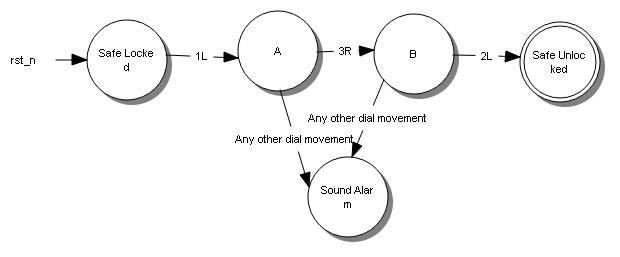
\includegraphics[scale=0.5]{img/03_safe_fsm.png}
	\end{frame}
	\begin{frame}{Finite State Machine}
    	\begin{itemize}
    	    \item More ways to represent finite state machine: transition table and a 5-tuple \{J, K, T, S, F\} (states, inputs, transition function, initial state, final states)
    	    \item Later in discussions of Unified Modeling Language (UML), we will find out that UML has also a state machine diagram
	    \end{itemize}
	\end{frame}
	\section{Petri Nets}
	\begin{frame}{Petri Nets}
    	\begin{itemize}
            \item Major difficulty with specifying concurrent systems is coping with timing.
            \item One technique to specifying systems with potential timing problems, is Petri nets.
            \item A petri-net consist of 4 parts:
            \begin{itemize}
                \item Set of places P
                \item Set of transitions T
                \item Input function I
                \item Output function O
            \end{itemize}
	    \end{itemize}
	\end{frame}
	\begin{frame}{Petri Nets: Example}
    	\begin{itemize}
            \item Set of places P is $\{p_1, p_2, p_3\}$
            \item Set of transitions T is $\{t_1, t_2\}$
            \item Input function $I(t_1) = \{p2, p4\}$ and $I(t_2) = \{p2\}$
            \item Output function $O(t_1) = \{p1\}$ and $O(t_2) = \{p3\}$
	    \end{itemize}
	    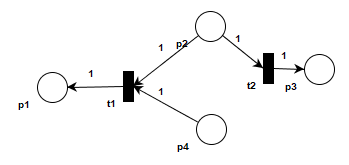
\includegraphics[scale=0.7]{img/03_petrinet_simple.png}
	\end{frame}
	\section{Z}
	\begin{frame}{Z}
    	\begin{itemize}
            \item Use of Z \cite{Spivey:1989:ZNR:61690} requires knowledge of set theory, functions, and discrete mathematics, including first-order logic.
            \item In this slide, we will use "The Elevator Problem" \cite[page 378]{Schach:2006:OCS:1207045} for use case
            \item In its simplest form, Z specification consists of:
            \begin{enumerate}
                \item Given sets, data types, and constants
                \item State definition
                \item Initial state
                \item Operations
            \end{enumerate}
	    \end{itemize}
	\end{frame}
	\begin{frame}{Z: 1 Given Sets}
    	\begin{itemize}
            \item Begins with a list of ``given sets''
            \item Name of such sets appear in brackets
            \item In elevator case, it is the \texttt{Button}, set of all buttons
            \item i.e. \texttt{[Button]}
            \item This \texttt{Button}, perhaps, is like a package name, since later we will meet a different one \texttt{button}
	    \end{itemize}
	\end{frame}
	\begin{frame}{Z: 2. State Definition}
    	\begin{itemize}
            \item Consists of a number of schemas (schemata)
            \item Each schema consists of a group of variable declarations and predicates that constrain the possible values of variables.
            \item In elevator case, there are four subsets of \texttt{Button}: floor buttons, elevator buttons, \texttt{buttons} (set of all buttons in case study), and pushed (set of buttons that have been pushed)
	    \end{itemize}
	    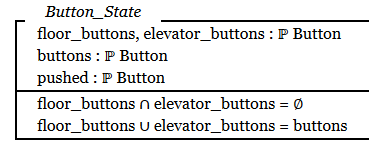
\includegraphics[scale=0.5]{img/03_z_button_state_schema.png}
	\end{frame}
	\begin{frame}{Z: 3. Initial State}
    	\begin{itemize}
            \item Abstract initial state describes the state when the system first is turned on.
            \item For elevator problem, the abstract initial state is as below.
	    \end{itemize}
	    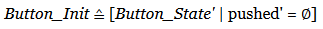
\includegraphics[scale=0.5]{img/03_z_initial_state.png}
    	\begin{itemize}
            \item This asserts that when the elevator system is first turned on, the set \texttt{pushed} initially is empty; i.e. all buttons are off.
	    \end{itemize}
	\end{frame}
	\begin{frame}{Z: 4. Operations}
    	\begin{itemize}
            \item If a button is pushed for the first time, then that button is turned on. It is depicted below.
	    \end{itemize}
	    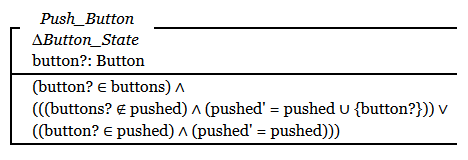
\includegraphics[scale=0.5]{img/03_z_push_button.png}
    	\begin{itemize}
            \item The following specification is for when an elevator arrives at a floor.
	    \end{itemize}
	    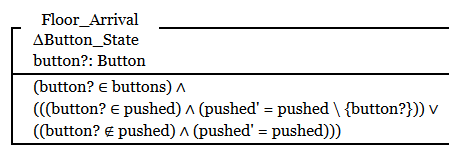
\includegraphics[scale=0.5]{img/03_z_floor_arrival.png}
	\end{frame}	
	\section{Comparison}
	\begin{frame}{Comparison of Classical Techniques}
	\begin{footnotesize}
        \begin{table}[]
        \centering
        \begin{tabular}{| p{1.5cm} | p{1.5cm} | p{2.5cm} | p{2.5cm} |}
        \hline
        \textbf{Method} & \textbf{Category} & \textbf{Strengths}                                                                                                                         & \textbf{Weakness}                                                                                            \\ \hline
Natural Language                   & Informal          & Easy to learn, use, and understand                                                               & Imprecise, specification can be ambiguous                           \\ \hline
Structured Analysis                & Semiformal        & Can be understood by client, more precise than informal                                          & Not as precise as formal techniques; generally cannot handle timing \\ \hline
Petri Nets \& Z                    & Formal            & Extremely precise; can reduce analysis faults, development cost; can support correctness proving & Hard to learn and use; almost impossible for client to understand   \\ \hline
        \end{tabular}
        \end{table}
        \end{footnotesize}
\end{frame}
	
	\section{References}
	\begin{frame}[allowframebreaks]
        \frametitle{References}
        \bibliographystyle{amsalpha}
        \bibliography{module_03}
	\end{frame}

\end{document}
\end